\documentclass[11pt, a4paper,titlepage]{article}
\usepackage[utf8]{inputenc}
\usepackage[T1]{fontenc}
\usepackage{fixltx2e}
\usepackage{graphicx}
\usepackage{longtable}
\usepackage{float}
\usepackage{wrapfig}
\usepackage{soul}
\usepackage{textcomp}
\usepackage{marvosym}
\usepackage{wasysym}
\usepackage{latexsym}
\usepackage{hyperref}
\usepackage{amssymb}
\usepackage{hyperref}
\usepackage[bottom]{footmisc}
\tolerance=1000
\usepackage[left=3.35cm, right=3.35cm, top=3.35cm, bottom=3.35cm]{geometry}
\usepackage[utf8]{inputenc}
\usepackage[greek,english]{babel}
\usepackage{graphicx}
\usepackage{titlesec}
\usepackage{tocbibind}
\makeatletter
\def\@seccntformat#1{%
  \expandafter\ifx\csname c@#1\endcsname\c@section\else
  \csname the#1\endcsname\quad
  \fi}
\makeatother
\begin{document}

\begin{titlepage}
  \begin{center}
    
    
\includegraphics[scale=1.5]{Figures/kuleuven_logo.pdf}~\\[4.5cm]
    
    \textsc{\Large Bio-Molecular Model Building}\\[0.5cm]
    
    % Title
    \rule{\linewidth}{0.3mm}\\[0.4cm]
    {\huge \bfseries Exam Exercise} \\[0.4cm]
    {\large Spring 2015} \\[0.4cm]
    \rule{\linewidth}{0.3mm}\\[1.5cm]
    
    % Author and supervisor
    \begin{minipage}{0.4\textwidth}
      \begin{flushleft} \large
        \emph{Author:}\\
        Cedric \textsc{Lood}\\
        Yi Ming \textsc{Gan}\\
      \end{flushleft}
    \end{minipage}
    \begin{minipage}{0.4\textwidth}
      \begin{flushright} \large
        \emph{Supervisors:} \\
        Prof. M. \textsc{De Maeyer}\\
        dr. J. \textsc{De Raeymaecker}\\
        dr. X. \textsc{Qing}
      \end{flushright}
    \end{minipage}
    
    \vfill
    
    
\includegraphics[scale=0.15]{Figures/KUL.jpg}~\\[0.5cm]

    % Bottom of the page
    {\large \today}
    
  \end{center}
\end{titlepage}

\setcounter{tocdepth}{3}

\tableofcontents
\newpage

\section*{Question 1}
\addcontentsline{toc}{section}{Question 1}
\subsection*{Part a}
\addcontentsline{toc}{subsection}{Part a}

Chain A is the kinase domain (CDK2), N-terminal is colored in blue and
C-terminal is colored in green.  The regulatory domain (cyclin-A2) is
chain B, colored in yellow.
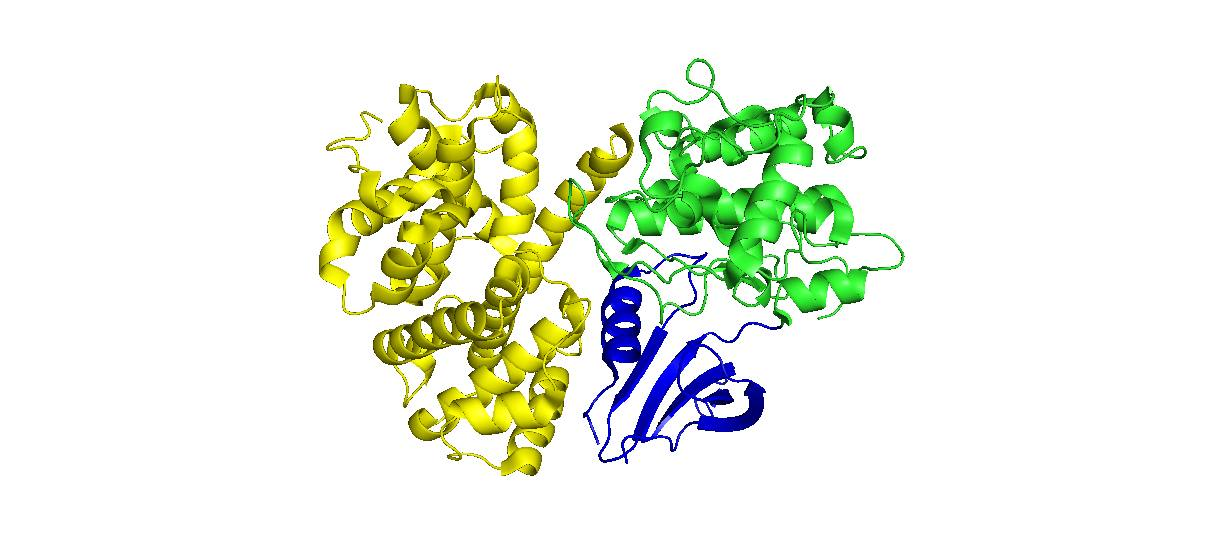
\includegraphics[width=15cm]{./Figures/1a.jpg}

\subsection*{Part b}
\addcontentsline{toc}{subsection}{Part a}

This is the list of residue sequences associated with their
corresponding secondary structures::
\begin{description}
\itemsep0em 
\item[N-Terminus]
\item[1-4] Loop
\item[5-11] Beta sheet
\item[12-16] Loop
\item[17-23] Beta sheet
\item[24-28] Loop
\item[29-36] Beta sheet
\item[37-45] Loop
\item[46-57] Alpha helix
\item[58-65] Loop
\item[66-71] Beta sheet
\item[72-74] Loop
\item[75-81] Beta sheet
\item[82-84] Loop
\item[C-Terminus]
\end{description}

\clearpage
And the topology diagram of the N-terminal domain:

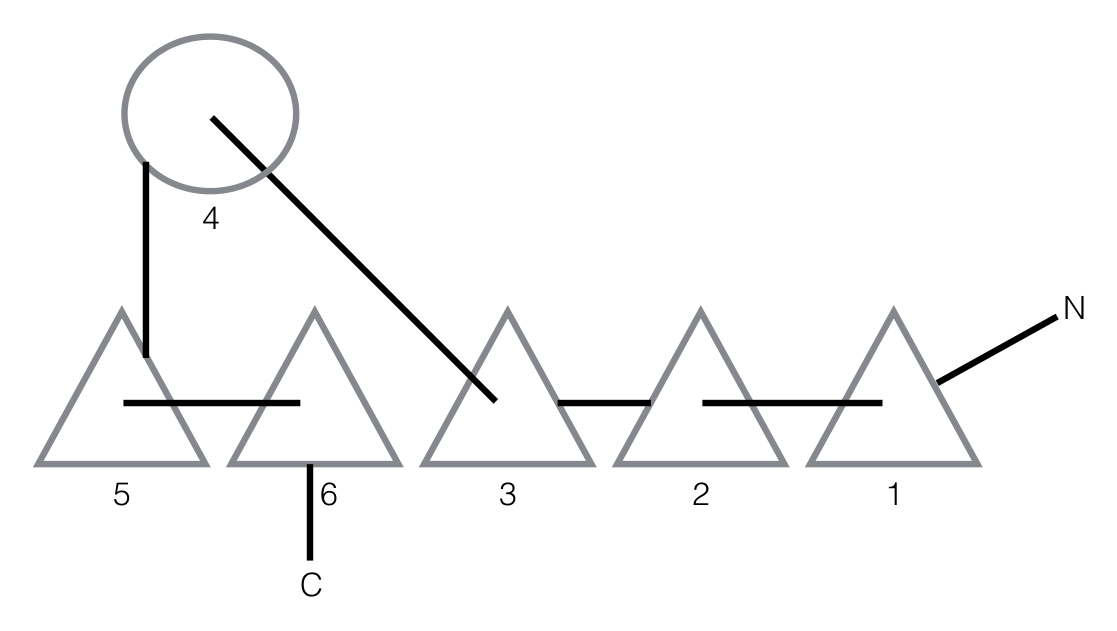
\includegraphics[width=12cm]{./Figures/1b.png}

\section*{Question 2}
\addcontentsline{toc}{section}{Question 2} The role of regulatory
domains in the kinases are to induce conformational changes that
switch the kinase from one form (inactive or active) to the other
\cite{ConformationalPlasticityKinases}.In the cartoon below, the red
structure is the 2SRC, the green one is 3LCK. A pfam analysis of 2SRC
reveals that the SH2 domain is located around positions TRP-148 to
TYR-230. This include the amino acids indicated on the second cartoon
figure below, namely ARG-155 and THR-179.

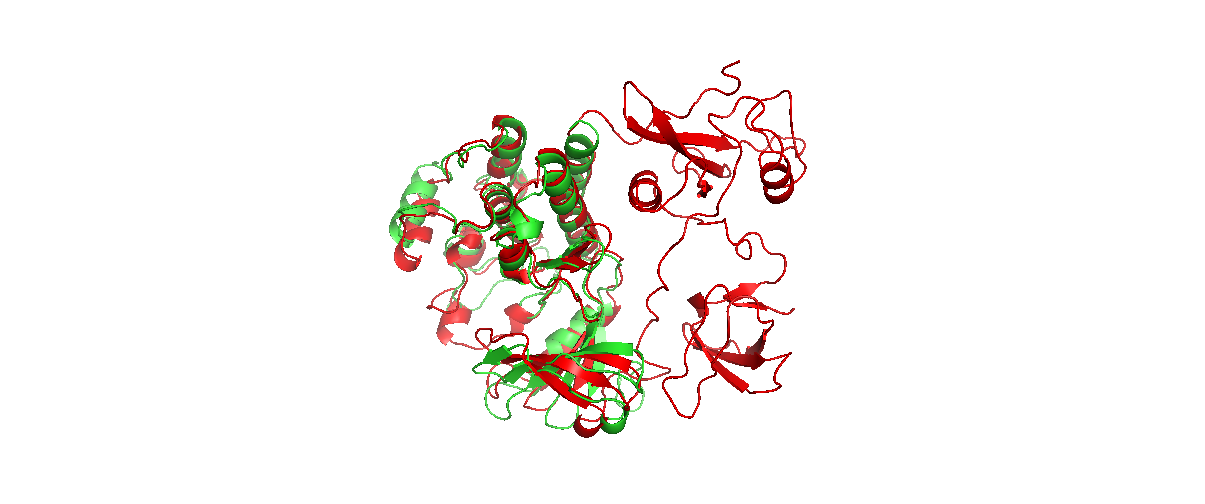
\includegraphics[width=15cm]{./Figures/2a.png}

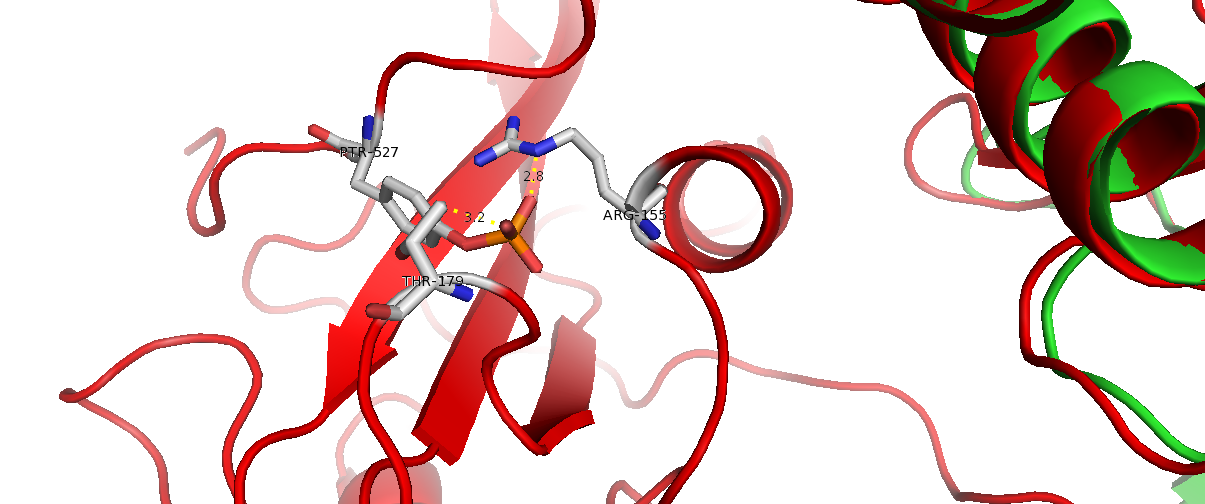
\includegraphics[width=15cm]{./Figures/2b.png}

\section*{Question 3}
\addcontentsline{toc}{section}{Question 3}
We extracted the data from the protein database using the following query:

\begin{verbatim}
Holdings : Molecule Type=ignore Experimental Method=X-RAY 

and 

DepositDateQuery: database_PDB_rev.date_original.comparator=between 
database_PDB_rev.date_original.min=2000-01-01 database_PDB_rev.date_original.max=2015-05-13 
database_PDB_rev.mod_type.comparator=< database_PDB_rev.mod_type.value=1 

and 

StructTitleQuery: struct.title.comparator=contains struct.title.value=Kinase
\end{verbatim}

We did export the results to a CSV file to further our analysis using
R and obtained the following summary table and associated graph:

\begin{verbatim}
> table(years) years 2000 2001 2002 2003 2004 2005 2006 2007 2008 2009
 2010 2011 2012 2013 2014 2015 41 84 91 131 123 192 224 298 329 309
 348 316 426 402 358 102 > barplot(table(years))
\end{verbatim}

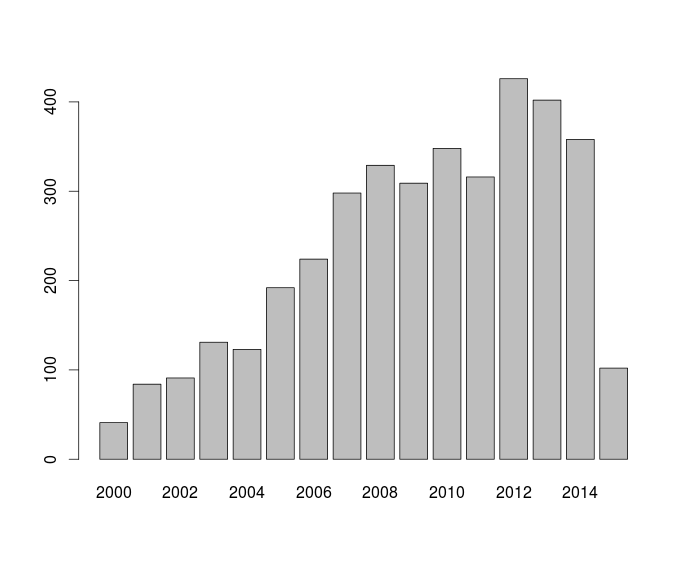
\includegraphics[width=12cm]{./Figures/pdb_kinases_growth.png}

We think that the steady increase in the number of kinases being
researched is linked to the fact that Kinases are involved in various
pathways whose defects lead to diseases. 

\section*{Question 4}
\addcontentsline{toc}{section}{Question 4}
\subsection*{Part a}
\addcontentsline{toc}{subsection}{Part a}

The molecule bound is Phosphoaminophosphonic Acid-Adenylate Ester, or
ANP. Along with 2 Magnesium Ions.

\subsection*{Part b}
\addcontentsline{toc}{subsection}{Part b}

ANP is an analog of ATP that cannot be hydrolized by the
kinase. Therefore it stays bound to the active site of the kinase and
allows for the crystal structure of the molecule to be established.

\subsection*{Part c}
\addcontentsline{toc}{subsection}{Part c}

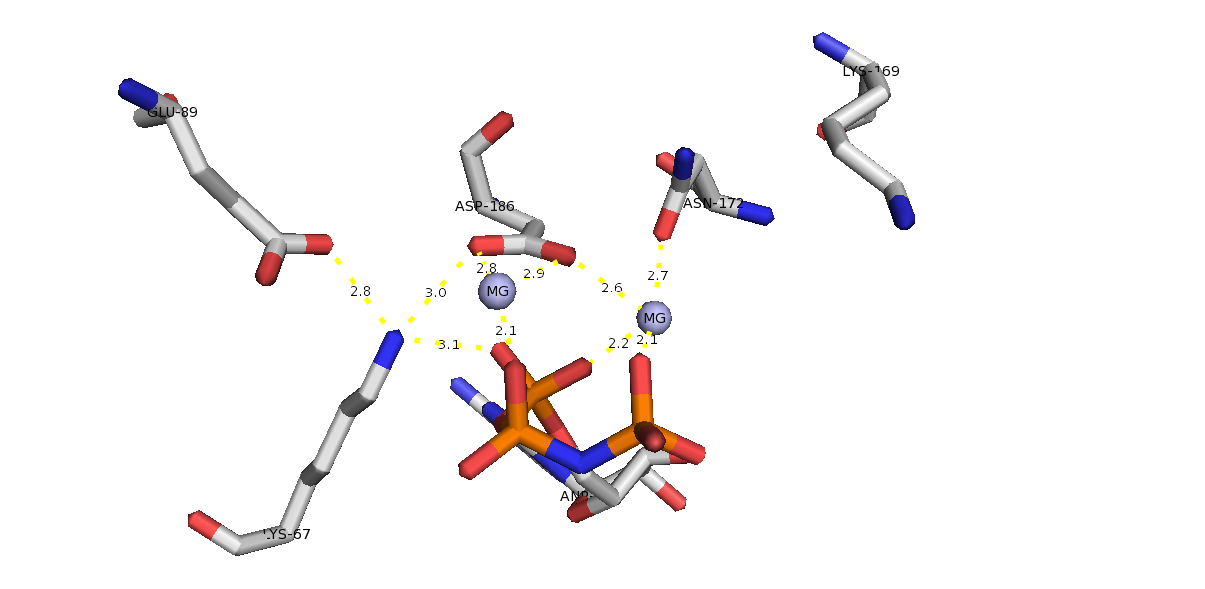
\includegraphics[width=15cm]{./Figures/4c.png}

As shown in the figure, a salt bridge is formed between Glu89 and
Lys67.  Lys67 forms a salt bridge directly with the $\alpha$-phosphate
oxygen of the ANP molecule. Asp186 forms H-Bond with the Lys67 and
also coordinates the Magnesium Ion, that in turns coordinates the
$\beta$-phosphate oxygen of the ANP molecule. Asn172, in collaboration
with Asp186 coordinates the second Magnesium Ion which interacts with
the $\alpha$ and $\gamma$-phosphate oxygens of the ANP molecule
\cite{CSPim1Kinase}.

\subsection*{Part d}
\addcontentsline{toc}{subsection}{Part d}

The AUTHOR section from the PDB file reveals the same list of names as
the list of the article's authors:

\begin{verbatim}
AUTHOR    K.C.QIAN,L.WANG,E.R.HICKEY,J.STUDTS,K.BARRINGER,C.PENG,               
AUTHOR   2 A.KRONKAITIS,J.LI,A.WHITE,S.MISCHE,B.FARMER         
\end{verbatim}
 
\section*{Question 5}
\addcontentsline{toc}{section}{Question 5}
We found 2 proteins of interest: 1JKK and 3F5U. Both have reasonable
resolutions and R-Free values are similar. 1JKK boasts a 'up to 1.5 A'
resolution of the catalytic domain. However, after visualizing the
B-Factors using pymol, we decided to go with 3F5U.

\subsection*{Part a}
\addcontentsline{toc}{subsection}{Part a}

The AUTHOR section from the PDB file reveals the same list of names as
the list of the article's authors:

\begin{verbatim}
AUTHOR    L.K.MCNAMARA,D.M.WATTERSON,J.S.BRUNZELLE
\end{verbatim}

\subsection*{Part b}
\addcontentsline{toc}{subsection}{Part b}

Arg156 and Glu107 have zero occupany. Since the orientation of the
residues in space could not be determined, the interaction of zero
occupancy residue with neighbouring residues is unknown. This may in
turn affect the protein model tertiary structure.  Gln223 has multiple
alternative rotamer conformations.

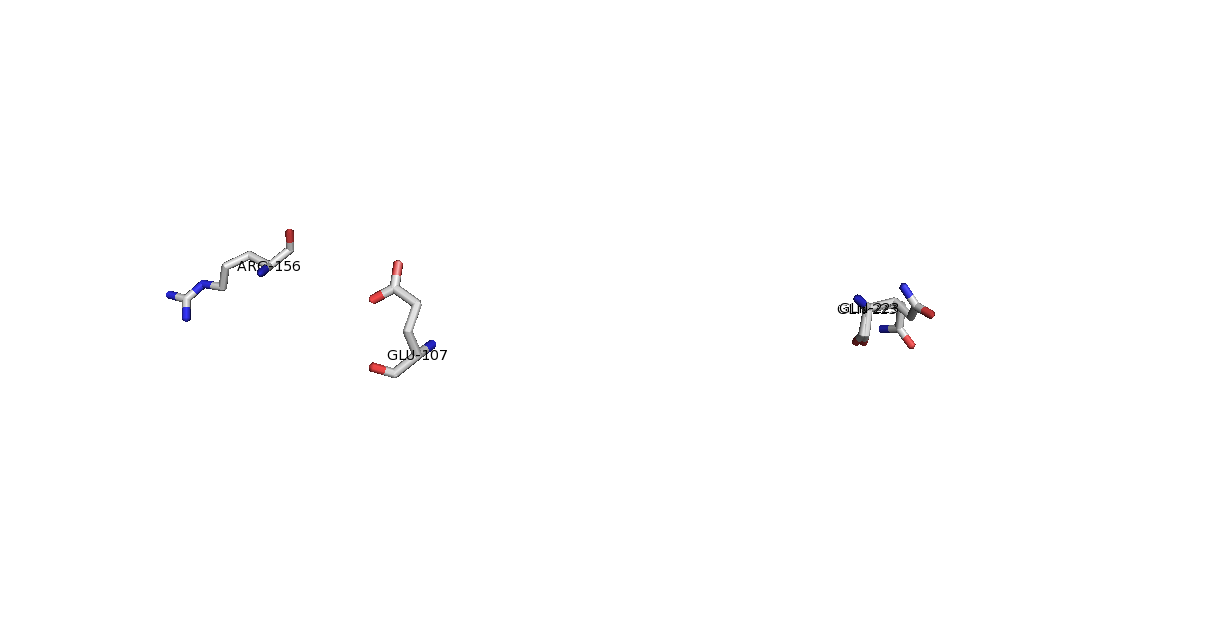
\includegraphics[width=15cm]{./Figures/5b.png}

\subsection*{Part c}
\addcontentsline{toc}{subsection}{Part c}

Overall, this structure has low B-factors. There is however a loop
region, located around amino acids 291-294, which displays higher
B-Factors (around 100). The reason for this seems to be lying in the
fact that this loop is part of a flexible regions at the C-Terminus,
which is not captured by the X-Ray crystalography.

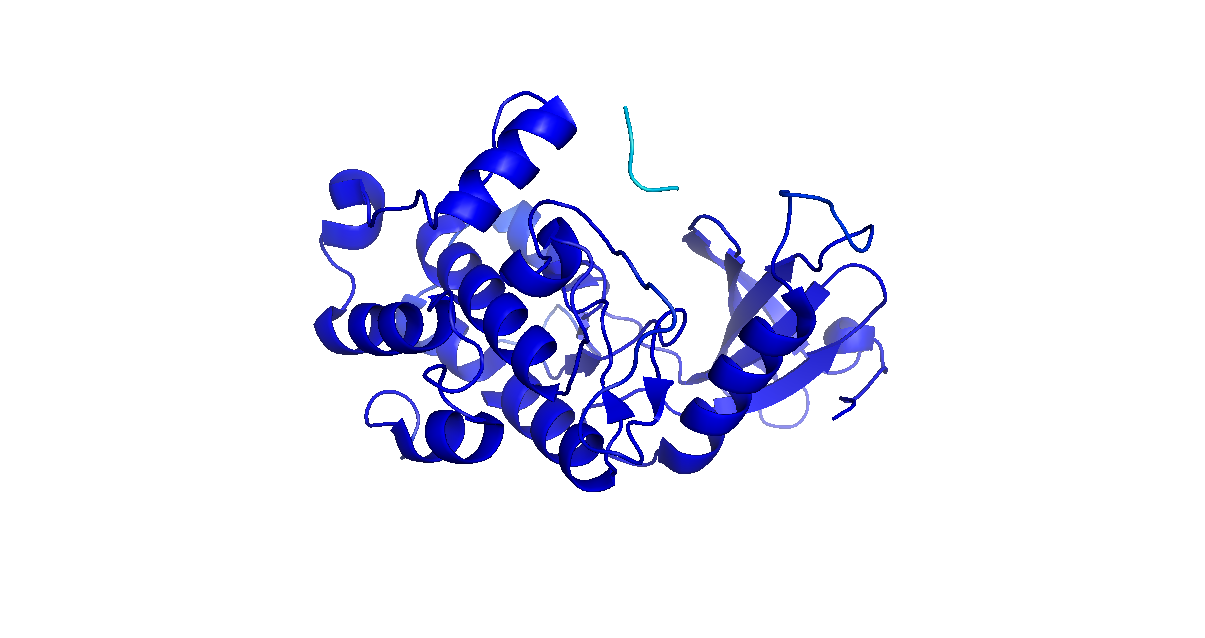
\includegraphics[width=15cm]{./Figures/5c.png}

\subsection*{Part d}
\addcontentsline{toc}{subsection}{Part d}

The domains present in DAPK1-Human
\footnote{\url{http://www.uniprot.org/uniprot/P53355}} are:

\begin{itemize}
\item Kinase whose function is to catalize the transfer of phosphate
  groups to specific substrates.
\item Ankyrin domains (multiple found) mediate protein-protein
  interactions.
  \footnote{\url{https://en.wikipedia.org/wiki/Ankyrin_repeat}}
\item Roc domain, which is a GTPase domain. GTP binding to the ROC
  domain activates kinase activity.
  \footnote{\url{http://www.copewithcytokines.de/cope.cgi?key=ROC\%20domain}} 
\item The death domain (DD) is a protein interaction module composed
  of a bundle of six alpha-helices. It is a
  Calcium/calmodulin-dependent serine/threonine kinase which acts as a
  positive regulator of apoptosis.
  \footnote{\url{http://www.deathdomain.org/proteins/search?term=DAPK1}}
\end{itemize}
\subsection*{Part e}
\addcontentsline{toc}{subsection}{Part e}

The sequences provided are all homologous and display sequence
similarity.Some of the organism in which the protein is found belong
to varied kingdom such as Animal, Bacteria, Plants, which indicates
that it must originates from an ancient gene that existed even before
the split between Eukaryotes and Prokaryotes on the tree of life.

To further our analysis, we used the guide tree created when we
performed the multiple sequence alignment, along with the results of
the alignment. We found that the gene had had multiple duplication
event during evolution. For example, we analyzed the duplication event
(indicated on the figure) that gave rise to the proteins indicated by
LRRK1, LRRK2, and LRRK3. All of which can be fount in organism
belonging to the Eukaryotic domain. On the picture below, you can see
that we emphasized 3 sub-clusters. The green and the red cluster show
the LRRK1 and LRRK2+LRRK3 groups (the blue cluster can be hypothesized
to have come from a duplication event early in the
Animals/Invertebrates branch).

Using the results from the sequence alignment, you can observe that
the alignment scores between the protein within the same cluster (for
example LRRK1) are better than the ones from another cluster (LRRK2 in
our example). This makes sense when you think about the evolutionary
distance between the 2 genes coding for these paralog genes.

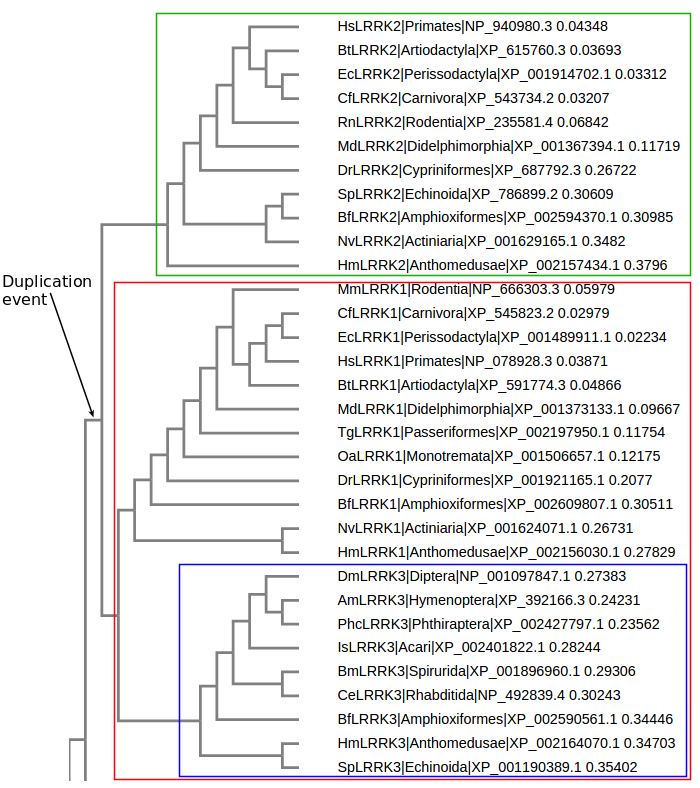
\includegraphics[width=17cm]{./Figures/5e.png}

\section*{Question 6}
\addcontentsline{toc}{section}{Question 6}
The essential features are indicated in the red frame on the cartoon
below. They are all hydrogen bridges.

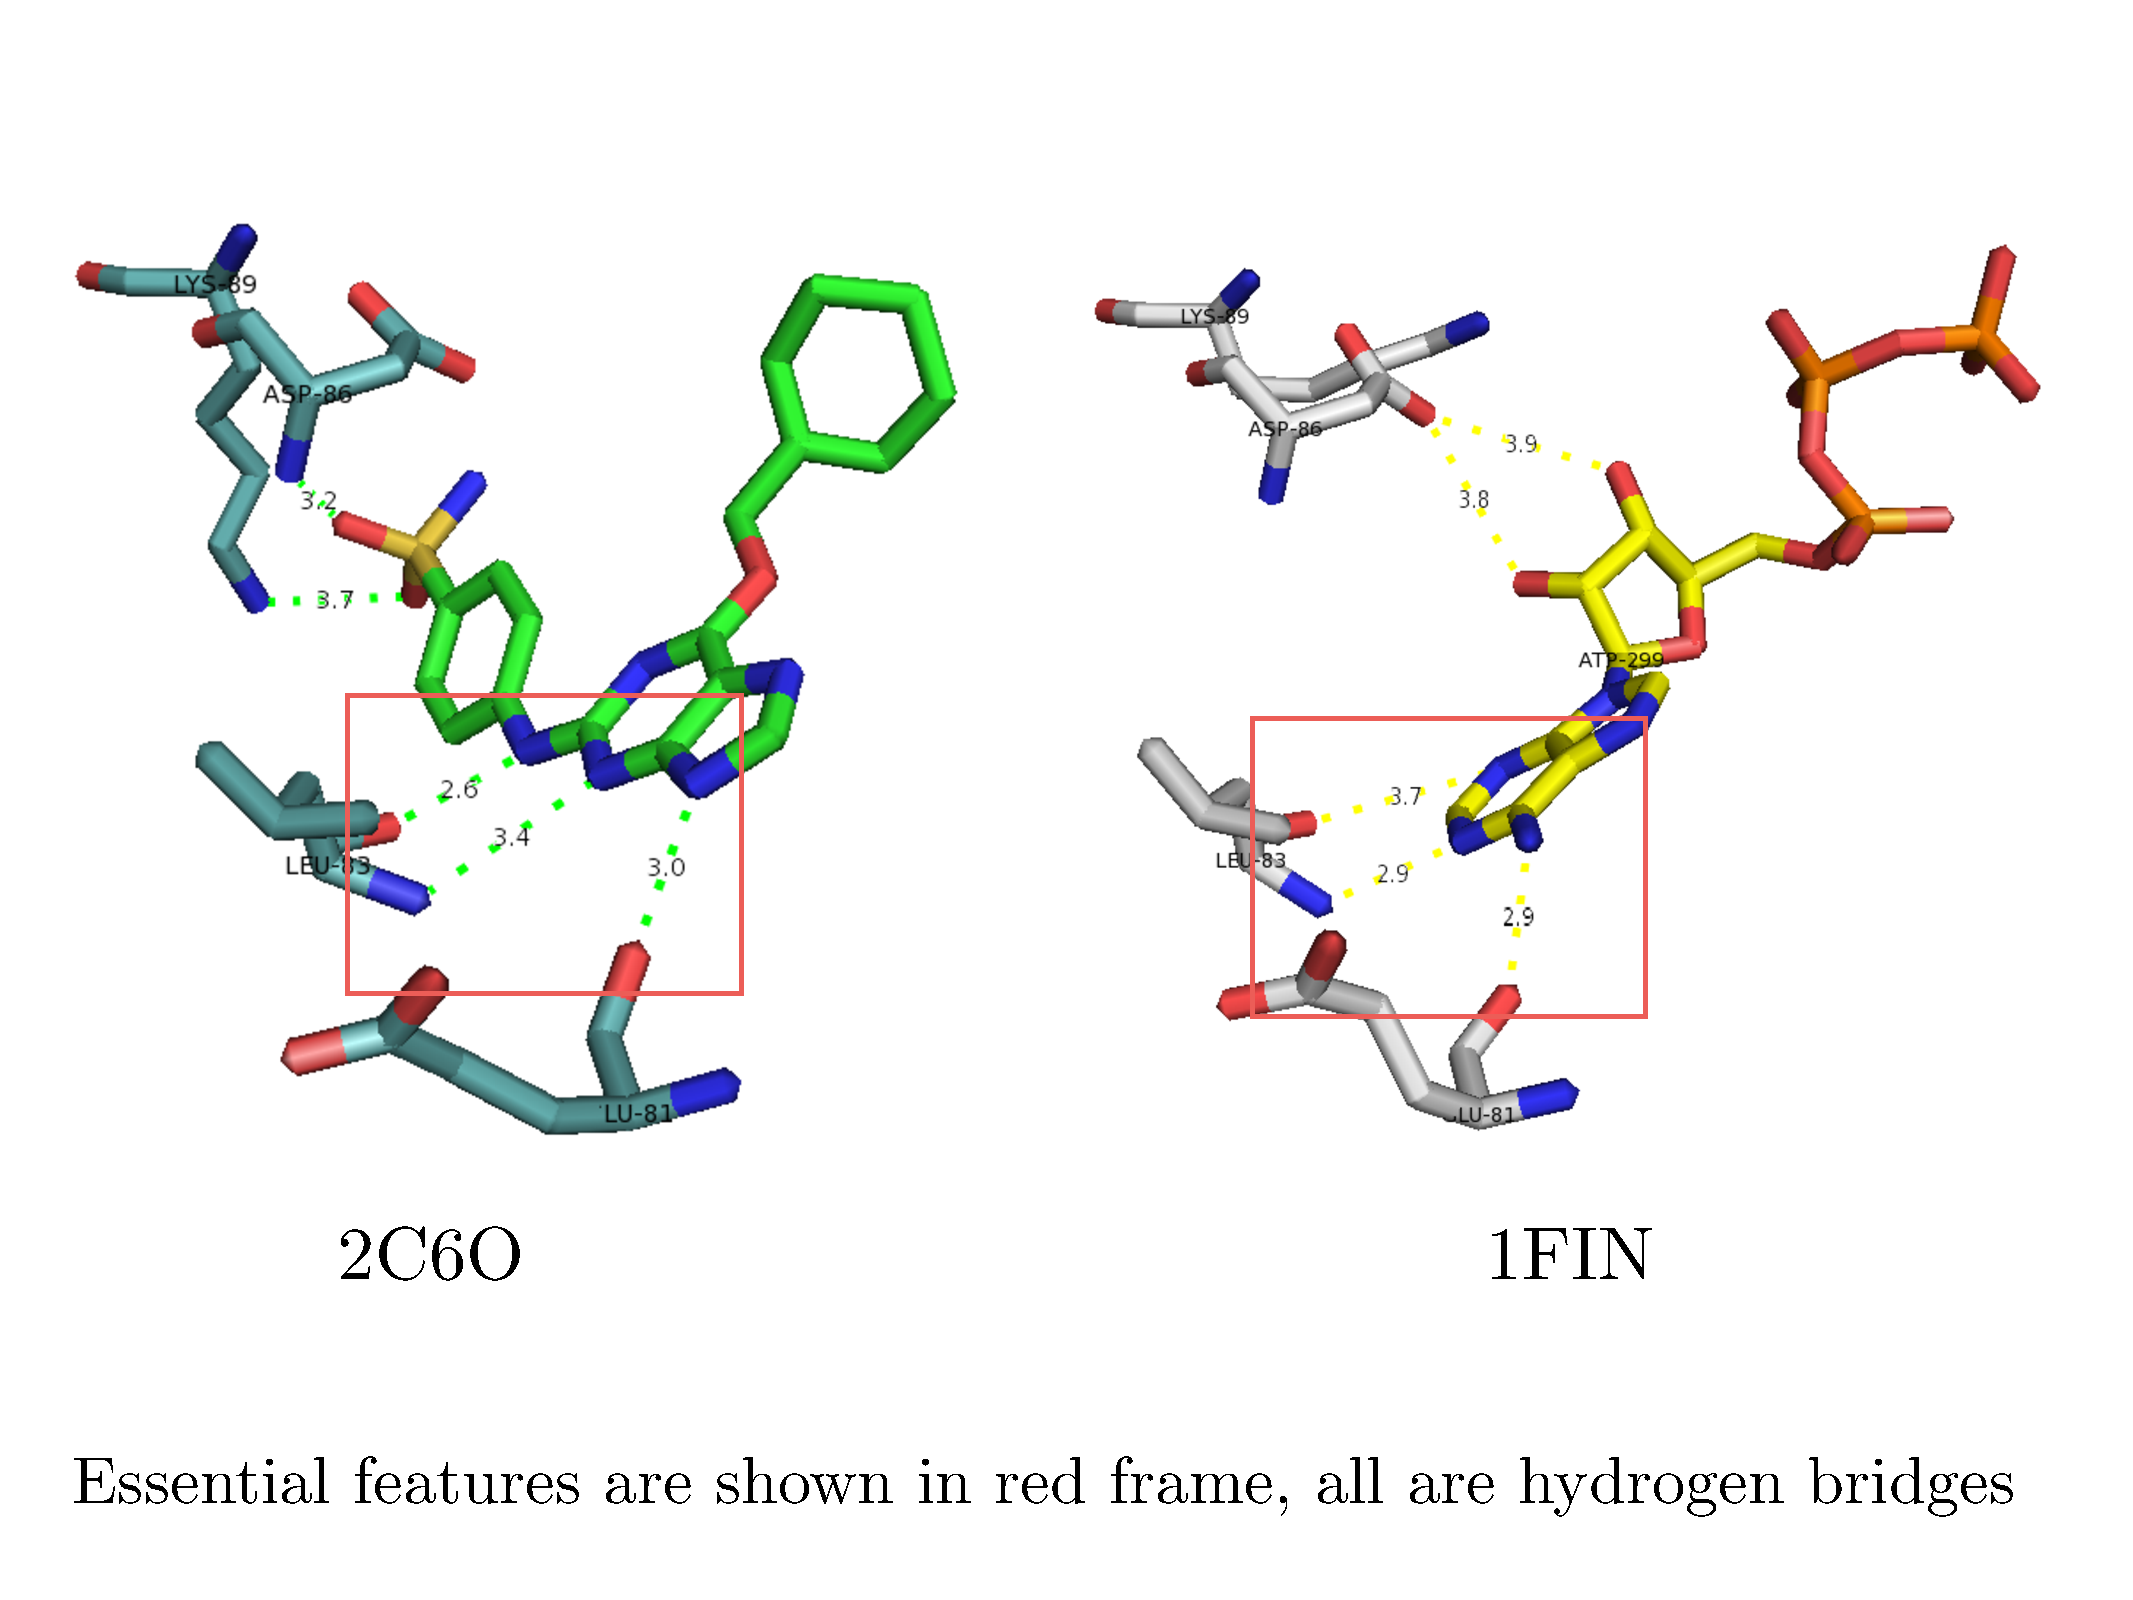
\includegraphics[width=17cm]{./Figures/6.pdf}

\section*{Question 7}
\addcontentsline{toc}{section}{Question 7}
\subsection*{Part a}
\addcontentsline{toc}{subsection}{Part a}

The following figure reports the selected model. We generated 5 of
them and selected the one which displayed the best properties. We paid
especially attention to the variable \emph{Number of residues in
  outlier region} and also to the \emph{GA341} and \emph{DOPE} scores
found in the \emph{model-single.log} report from the Modeller
software.

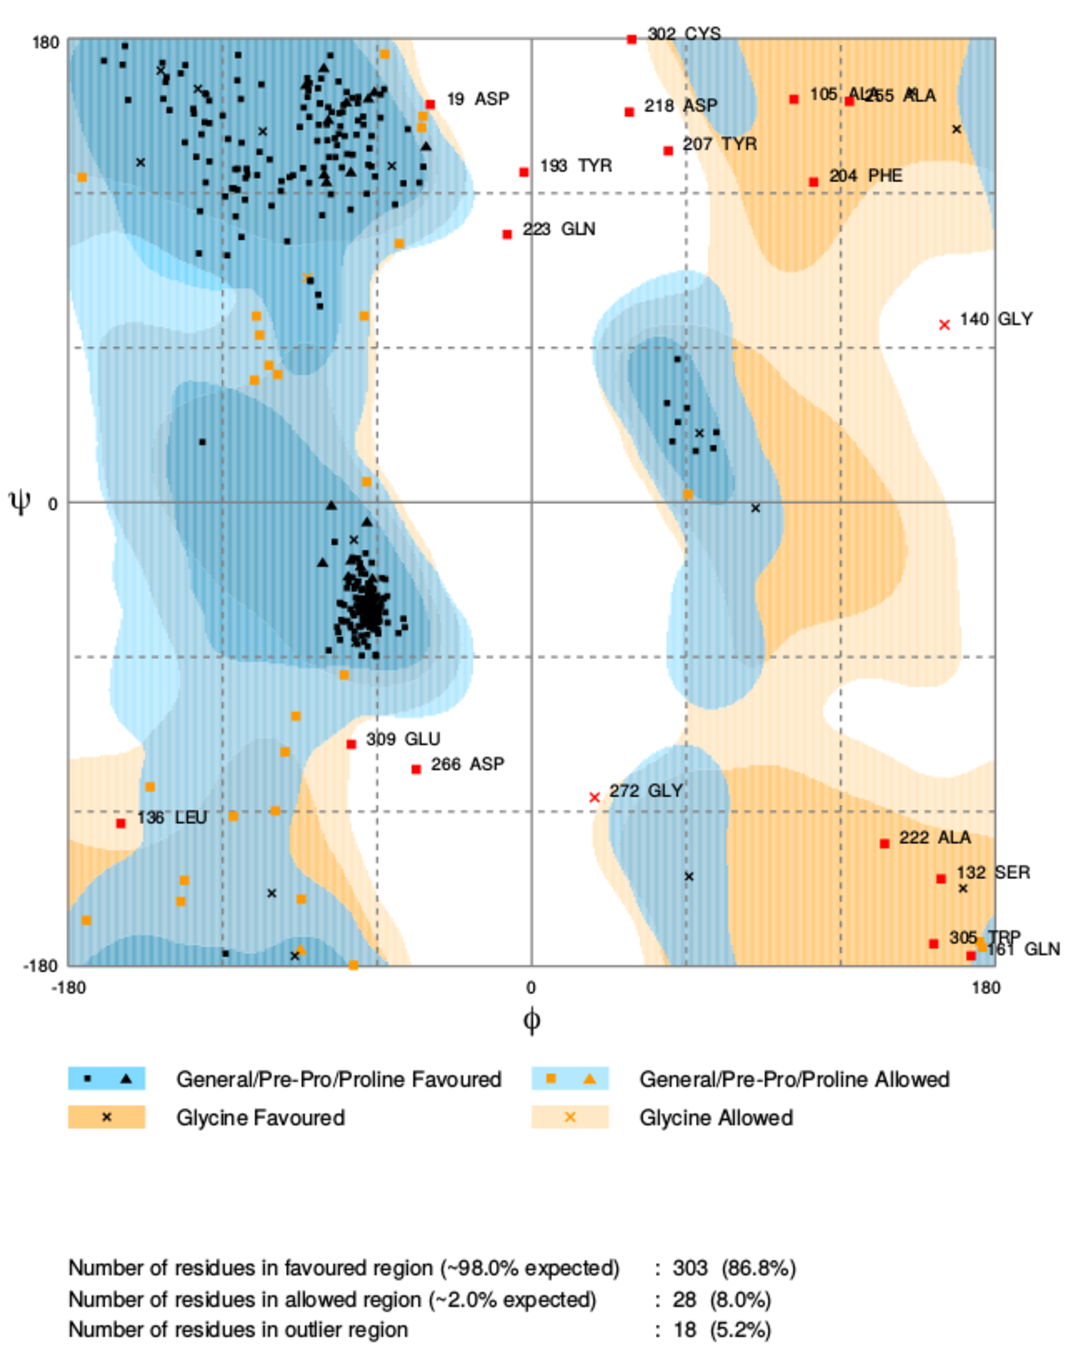
\includegraphics[width=16cm]{./Figures/7a-ramachandran.pdf}
\subsection*{Part b}
\addcontentsline{toc}{subsection}{Part b}

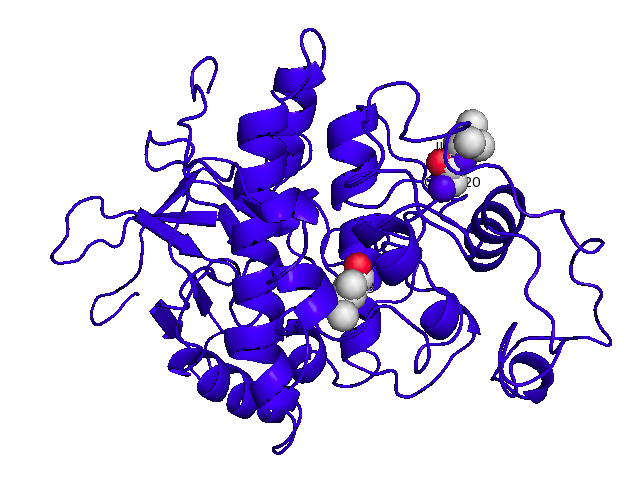
\includegraphics[width=10cm]{./Figures/7b.png}

\begin{verbatim}
CLUSTAL 2.1 multiple sequence alignment

lrrk2_mut2      ICGEGETLLKKWALYSFNDGEEHQKILLDDLMKKAEEGDLLVNPDQPRLTIPISQIAPDL 60
lrrk2_mut3      ICGEGETLLKKWALYSFNDGEEHQKILLDDLMKKAEEGDLLVNPDQPRLTIPISQIAPDL 60
lrrk2_wt        ICGEGETLLKKWALYSFNDGEEHQKILLDDLMKKAEEGDLLVNPDQPRLTIPISQIAPDL 60
lrrk2_mut1      ICGEGETLLKKWALYSFNDGEEHQKILLDDLMKKAEEGDLLVNPDQPRLTIPISQIAPDL 60
                ************************************************************

lrrk2_mut2      ILADLPRNIMLNNDELEFEQAPEFLLGDGSFGSVYRAAYEGEEVAVKIFNKHTSLRLLRQ 120
lrrk2_mut3      ILADLPRNIMLNNDELEFEQAPEFLLGDGSFGSVYRAAYEGEEVAVKIFNKHTSLRLLRQ 120
lrrk2_wt        ILADLPRNIMLNNDELEFEQAPEFLLGDGSFGSVYRAAYEGEEVAVKIFNKHTSLRLLRQ 120
lrrk2_mut1      ILADLPRNIMLNNDELEFEQAPEFLLGDGSFGSVYRAAYEGEEVAVKIFNKHTSLRLLRQ 120
                ************************************************************

lrrk2_mut2      ELVVLCHLHHPSLISLLAAGIRPRMLVMELASKGSLDRLLQQDKASLTRTLQHRIALHVA 180
lrrk2_mut3      ELVVLCHLHHPSLISLLAAGIRPRMLVMELASKGSLDRLLQQDKASLTRTLQHRIALHVA 180
lrrk2_wt        ELVVLCHLHHPSLISLLAAGIRPRMLVMELASKGSLDRLLQQDKASLTRTLQHRIALHVA 180
lrrk2_mut1      ELVVLCHLHHPSLISLLAAGIRPRMLVMELASKGSLDRLLQQDKASLTRTLQHRIALHVA 180
                ************************************************************

lrrk2_mut2      DGLRYLHSAMIIYRDLKPHNVLLFTLYPNAAIIAKIADYSIAQYCCRMGIKTSEGTPGFR 240
lrrk2_mut3      DGLRYLHSAMIIYRDLKPHNVLLFTLYPNAAIIAKIADYGTAQYCCRMGIKTSEGTPGFR 240
lrrk2_wt        DGLRYLHSAMIIYRDLKPHNVLLFTLYPNAAIIAKIADYGIAQYCCRMGIKTSEGTPGFR 240
lrrk2_mut1      DGLRYLHSAMIIYRDLKPHNVLLFTLYPNAAITAKIADYGIAQYCCRMGIKTSEGTPGFR 240
                ******************************** ******. *******************

lrrk2_mut2      APEVARGNVIYNQQADVYSFGLLLYDILTTGGRIVEGLKFPNEFDELEIQGKLPDPVKEY 300
lrrk2_mut3      APEVARGNVIYNQQADVYSFGLLLYDILTTGGRIVEGLKFPNEFDELEIQGKLPDPVKEY 300
lrrk2_wt        APEVARGNVIYNQQADVYSFGLLLYDILTTGGRIVEGLKFPNEFDELEIQGKLPDPVKEY 300
lrrk2_mut1      APEVARGNVIYNQQADVYSFGLLLYDILTTGGRIVEGLKFPNEFDELEIQGKLPDPVKEY 300
                ************************************************************

lrrk2_mut2      GCAPWPMVEKLIKQCLKENPQERPTSAQVFDILNSAELVCLTRRILLPKNV 351
lrrk2_mut3      GCAPWPMVEKLIKQCLKENPQERPTSAQVFDILNSAELVCLTRRILLPKNV 351
lrrk2_wt        GCAPWPMVEKLIKQCLKENPQERPTSAQVFDILNSAELVCLTRRILLPKNV 351
lrrk2_mut1      GCAPWPMVEKLIKQCLKENPQERPTSAQVFDILNSAELVCLTRRILLPKNV 351
                ***************************************************
\end{verbatim}
\subsection*{Part c}
The multiple sequence alignment below reveals mutations in the Amino
Acids at position 212, 219, and 220, also indicated in the cartoon as
spheres. These mutations convert hydrophobic amino acids (Iso, Gly) to
polar amino acids (Ser, Thr) who are prone to establish H-bonds,
making the transition to the active or inactive form of the molecule
more difficult.by reducing the flexibility of the region.

\bibliographystyle{plain} \bibliography{bib-db}
\end{document}
